\documentclass[10pt]{beamer}

\usepackage{verbatim}
\usepackage{graphicx,color}
\usepackage[french]{babel}
\usepackage{xspace}
\usepackage{tikz}

\usecolortheme{rose}
\setbeamertemplate{footline}{}
\setbeamertemplate{navigation symbols}{}
\setbeamercovered{invisible}
 
\usepackage{fontspec}

\setsansfont{PalatinoSansLTPro}[
   Path = /home/charles/charles_work/fonts/PalatinoSans/, 
   Extension      = .otf,
   UprightFont    = *-Regular,
   BoldFont= *-Bold ,
   ItalicFont = *-Italic,
   BoldItalicFont = *-BoldIta
]




\title[Introduction à la Sécurité]{Introduction à la Sécurité}

\subtitle{Organisation}
\author[C. Bouillaguet]{\textbf{Charles Bouillaguet / Ninon Devis}}
\institute[SU]{Sorbonne Université}

\date{ISEC}

\begin{document}
%\maketitle

\begin{frame}
  
  \centering

  \scalebox{6}{\bfseries \alert{Welcome !}}
  
  \vspace{1cm}
  
  \textbf{\Large Introduction au Calcul Haute Performance : Notions de Base}

  \bigskip

  a.k.a. MU4I903 (Masters Universitaires) a.k.a. N8-IPA (MAIN4)
\end{frame}

%%%%%%%%%%%%%%%%%%%%%%%%%%%%%%%%%%%%%%%%%%%%%%%%%%%%%%%%%%%%%%%%%%%%%%%%%%%%%%%%%

\begin{frame}
  \frametitle{Organisation de l'UE}

  \begin{block}{Documents, planning, etc.}
    Tout est sur Moodle !!
  \end{block}
  
  \begin{itemize}
  \item 10 semaines
  \item 1 semaine = cours + TD/TP (en principe)
  \item Pas d'examen réparti au milieu (\og partiel \fg)
  \item Gros projet
  \item Deux rendus : un à mi-semestre, un à la fin
  \end{itemize}
\end{frame}

%%%%%%%%%%%%%%%%%%%%%%%%%%%%%%%%%%%%%%%%%%%%%%%%%%%%%%%%%%%%%%%%%%%%%%%%%%%%%%%%%


\begin{frame}
  \begin{alertblock}{Équipe pédagogique}
    \begin{description}
    \item[Cours] ~ 
      \begin{itemize}    
      \item Charles Bouillaguet (SU)
      \end{itemize}
      
    \item[TD/TP (SFPN/IQ/...)] ~ 
      \begin{itemize}    
      \item Vincent Neiger (SU)
      \end{itemize}

    \item[TD/TP (MAIN4)] ~ 
      \begin{itemize}
      \item Charles Bouillaguet (SU)
      \end{itemize}
    \end{description}
  \end{alertblock}
\end{frame}



%%%%%%%%%%%%%%%%%%%%%%%%%%%%%%%%%%%%%%%%%%%%%%%%%%%%%

\begin{frame}[label=tme]
  \frametitle{Concept des Travaux sur Machine Encadrés}

  \begin{columns}
    \begin{column}{7cm}

      \begin{block}{Pratiquer la programmation parallèle}
        \begin{itemize}
        \item Vous avez tous un cluster chez vous ?
        \end{itemize}
      \end{block}

      \medskip

      \begin{alertblock}<2->{\textbf{Pas de cluster à la maison ?}}
        \begin{itemize}
        \item Dommage !
        \end{itemize}
      \end{alertblock}
      
      \medskip

      \begin{exampleblock}<3->{Heureusement, on a un plan B}
        \begin{itemize}
        \item Grid'5000
        \end{itemize}
      \end{exampleblock}
      
    \end{column}
    \begin{column}{4cm}
    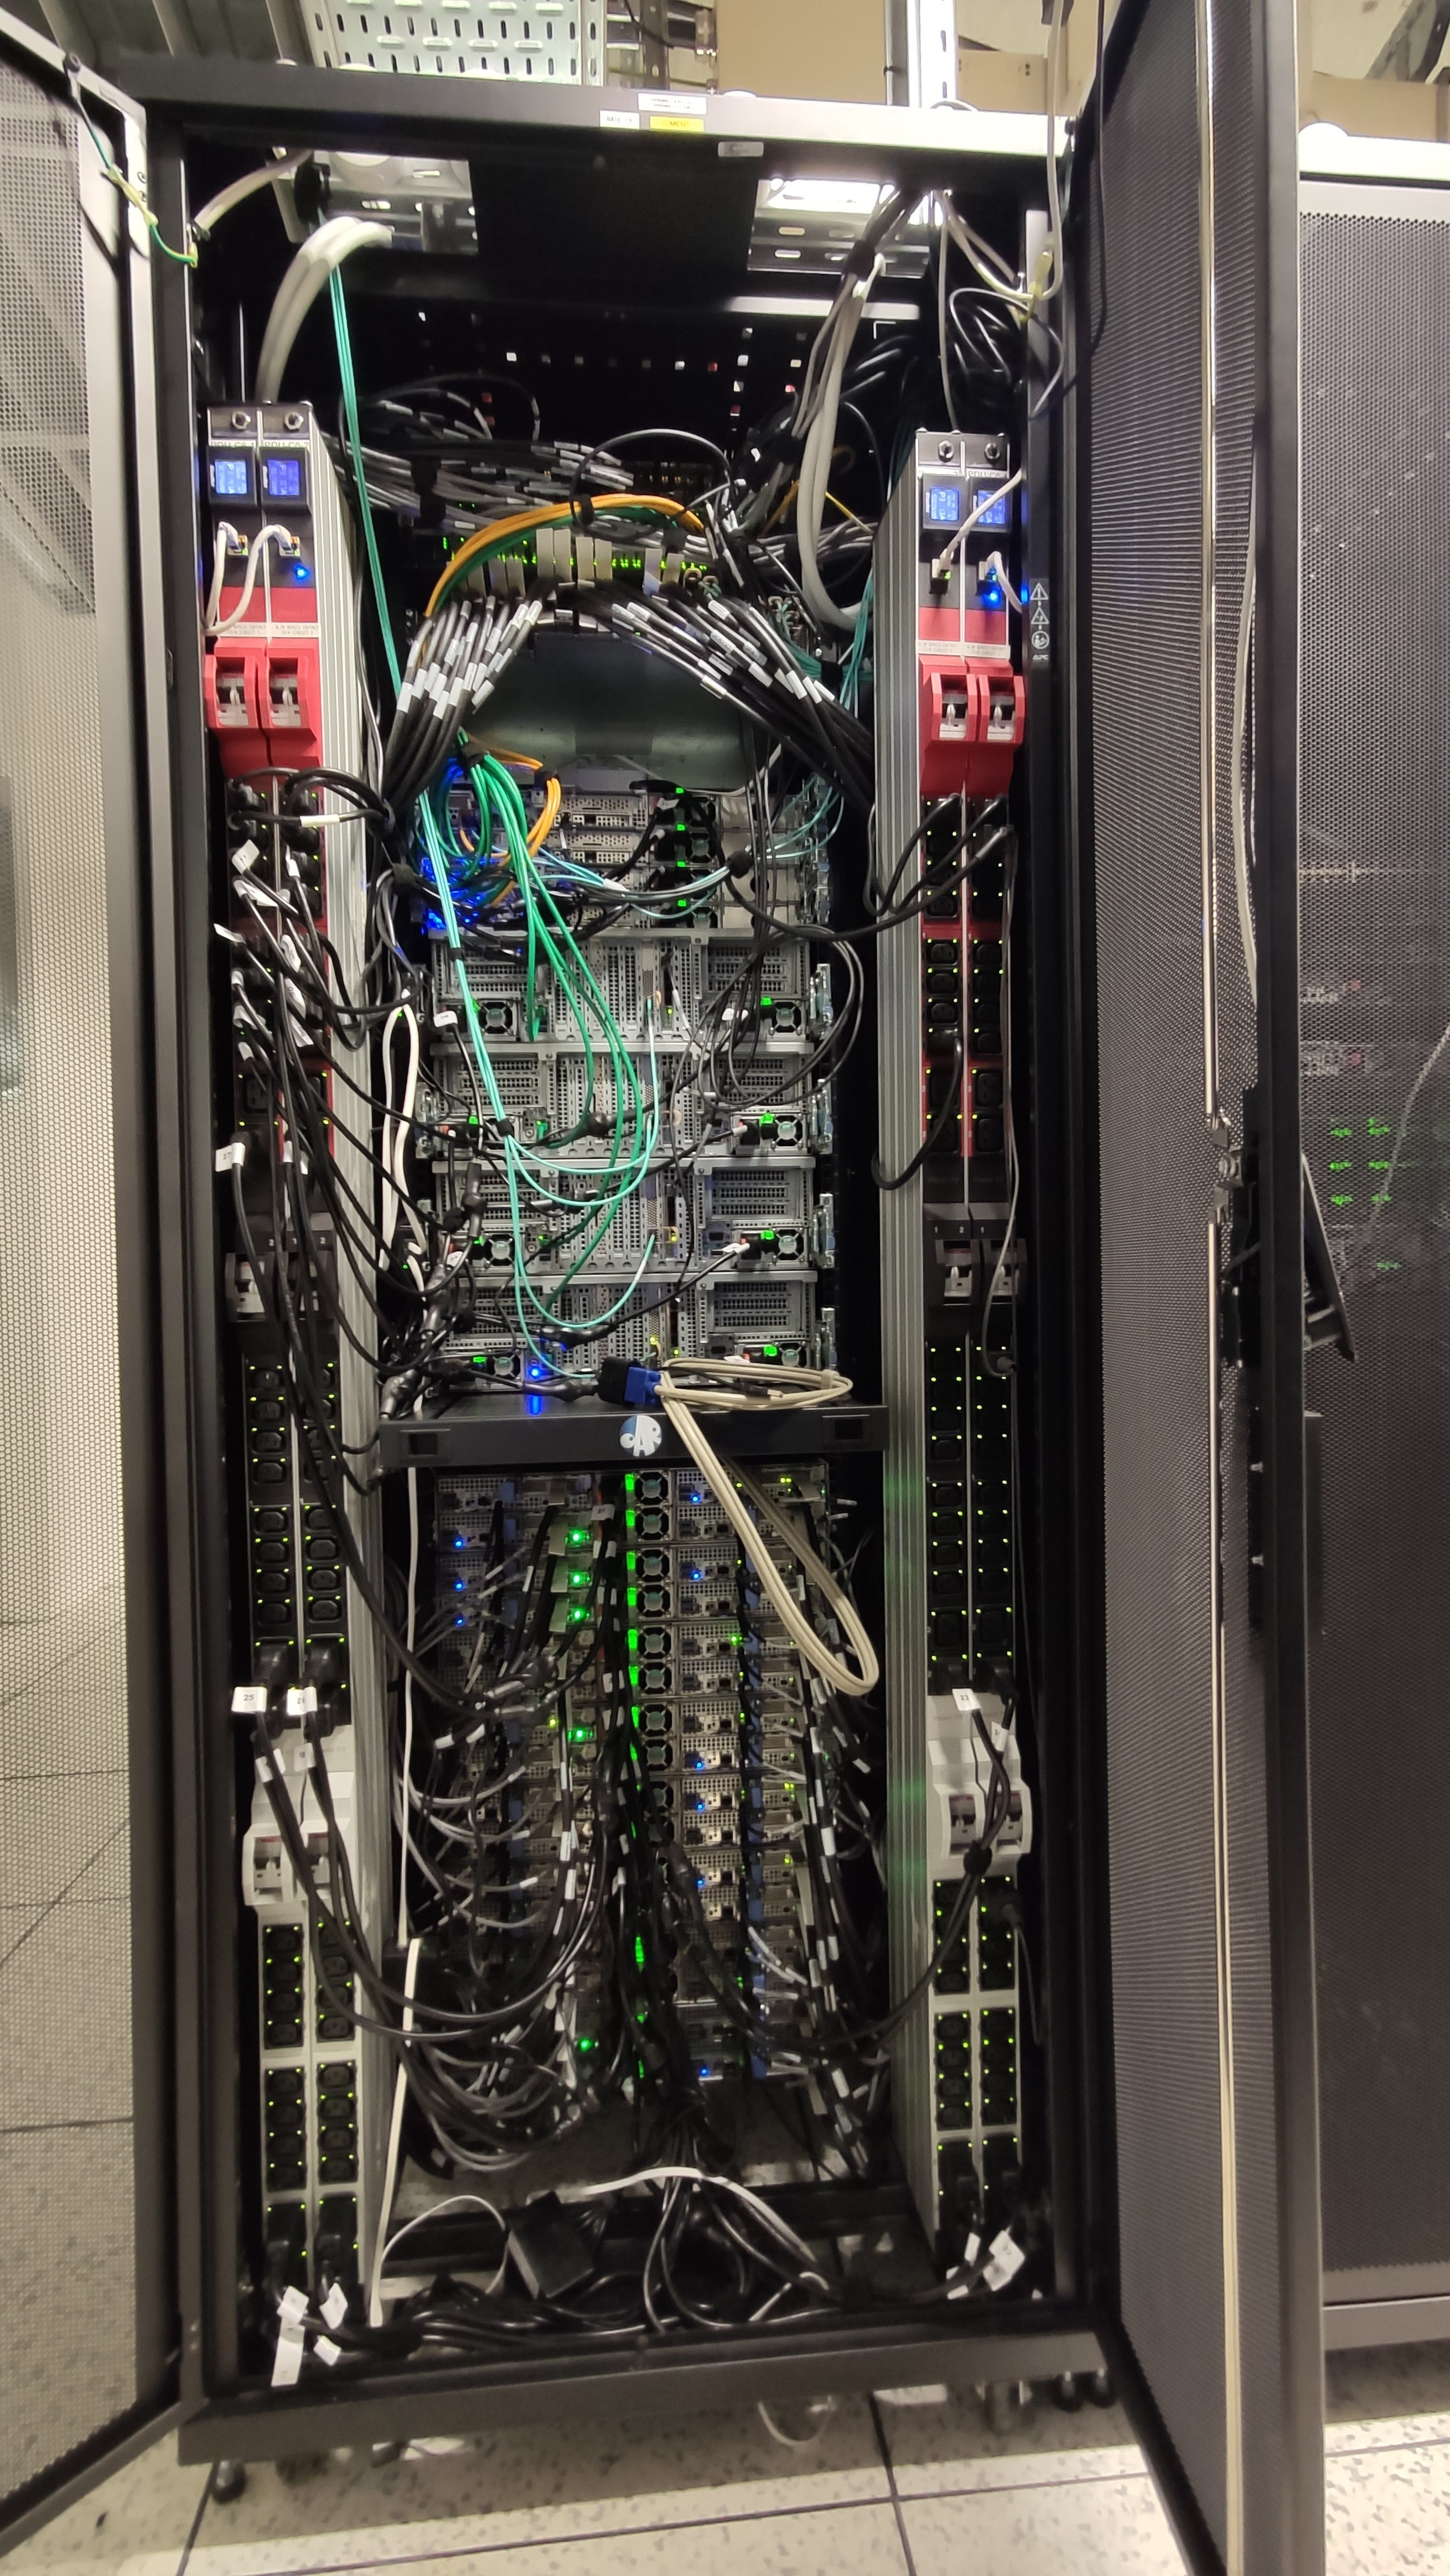
\includegraphics[height=8cm]{cluster.jpg}
  \end{column}
\end{columns}
\end{frame}

%%%%%%%%%%%%%%%%%%%%%%%%%%%%%%%%%%%%%%%%%%%%%%%%%%%%%

\begin{frame}[label=tme]
  
\includegraphics{grid5000_logo.png}

  \begin{columns}
    \begin{column}{5cm}

      \begin{exampleblock}{C'est quoi ?}
        \begin{itemize}
        \item Infrastructure publique de recherche
        \item Mutualisation de ressources de calcul
        \end{itemize}
      \end{exampleblock}
      
      \begin{block}{Les détails}
        \begin{itemize}
        \item 8 sites
        \item 37 clusters
        \item 806 ``ordinateurs''
        \item 15 702 coeurs en tout
        \end{itemize}
      \end{block}

      %%%%%%%%%%%%
      
    \end{column}
    \begin{column}{7cm}
      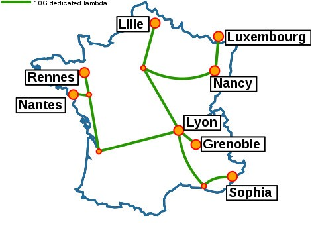
\includegraphics[width=7cm]{grid5000.pdf}
    \end{column}
  \end{columns}
\end{frame}

%%%%%%%%%%%%%%%%%%%%%%%%%%%%%%%%%%%%%%%%%%%%%%%%%%%%%

\begin{frame}[label=tme]
  \frametitle{
\includegraphics[height=1cm]{grid5000_logo.png}}

  \begin{block}{Accès à distance via \textbf{ssh}}
    \begin{enumerate}
    \item Connection à un \textbf{serveur d'accès} de Grid'5000
      \begin{itemize}
      \item \texttt{ssh login@access.grid5000.fr}
      \end{itemize}

      \smallskip
      
    \item Connection à la \textbf{frontale} d'un \textbf{site}
      \begin{itemize}
      \item \texttt{ssh nancy}
      \end{itemize}

      \smallskip
      
    \item Réservation des \textbf{noeuds de calcul} via \textbf{OAR}
      \begin{itemize}
      \item \texttt{oarsub --interactive --property "cluster='gros'"}
      \end{itemize}

      \smallskip
      
    \item Hop ! Connecté à un noeud de \texttt{gros}
      \begin{itemize}
      \item 18 coeurs à 2.2Ghz, 96Go de RAM, 25Gbps ethernet
      \end{itemize}
    \end{enumerate}
  \end{block}

  \begin{alertblock}{Conditions d'utilisation}
    \begin{itemize}
    \item Ne pas monopoliser les ressources
    \item Ne pas miner de cryptomonnaies (même ``pour la science'')
    \end{itemize}
  \end{alertblock}
\end{frame}

%%%%%%%%%%%%%%%%%%%%%%%%%%%%%%%%%%%%%%%%%%%%%%%%%%%%%

\begin{frame}[label=tme]
  \frametitle{
\includegraphics[height=1cm]{grid5000_logo.png}}

  \begin{alertblock}{Votre \textbf{devoir}}
    \begin{itemize}
    \item Lire la doc sur \url{https://www.grid5000.fr}
    \item Relire la doc, rerelire la doc, rerererelire la doc
    \item Ça m'\textbf{énerve} qu'on me pose une question alors que la doc contient la réponse
    \item Mais \textbf{n'hésitez pas} à nous poser des questions !
    \end{itemize}
  \end{alertblock}
  
  \medskip
  
  \begin{exampleblock}{Bon à savoir}
    \begin{itemize}
    \item Les \texttt{\$HOMEDIR} ne sont pas les mêmes d'un site à l'autre
    \item Fonctionnement jour/nuit et semaine/week-end
    \item \textbf{OAR} : interactif, \emph{batch} ou réservation
    \item Les autres utilisateurs aussi peuvent réserver les ressources
    \end{itemize}
  \end{exampleblock}

\end{frame}

%%%%%%%%%%%%%%%%%%%%%%%%%%%%%%%%%%%%%%%%%%%%%%%%%%%%%%%%%%%%%%%%

\begin{frame}
  \begin{block}{Le projet}
    \begin{itemize}
    \item \textbf{Pratique} = partie importante de l'apprentissage du HPC

      \medskip
      
    \item \textbf{Concept} :
      \begin{itemize}
      \item On vous fourni un code \textbf{séquentiel}
      \item Vous devez en faire une (ou des) versions \textbf{parallèles}
      \item Évaluer les \textbf{performances}
      \item Résoudre des \textbf{instances défi}
      \item Rédiger un \textbf{rapport}
      \end{itemize}
  
      \medskip

    \item \textbf{Quantité de travail nécessaire} : pas négligeable \includegraphics[width=0.5cm,trim=0 17mm 0 0]{triste}
      
      \medskip
      
    \item \textbf{Planning} :
      \begin{itemize}
      \item 50\% du semestre : rendu 1ère version
      \item 50\% + $\varepsilon$ du semestre : retours sur les rendus
      \item 100\% du semestre : rendu 2ème version
      \end{itemize}
    \end{itemize}
  \end{block}

  \medskip
  
  \centering 
\url{http://hpc.sfpn.net/static/project.py}
 
\end{frame}

%%%%%%%%%%%%%%%%%%%%%%%%%%%%%%%%%%%%%%%%%%%%%%%%%%%%%%%%%%%%%%%%%%%%%%%

\begin{frame}
  \begin{block}{Évaluation de l'UE}
    \begin{itemize}
    \item \textbf{Examen final} 
      \begin{itemize}
      \item Vendredi 20 mai
      \end{itemize}

      \medskip
      
    \item \textbf{Projet} 
      \begin{itemize}
      \item 1ère version le 18 mars
      \item 2ème version le 20 mai
      \end{itemize}
      
      \medskip
      
    \item Note finale : moyenne des deux
    \end{itemize}
  \end{block}
\end{frame}

%%%%%%%%%%%%%%%%%%%%%%%%%%%%%%%%%%%%%%%%%%%%%%%%%%%%%%%%%%%%%%%%%%%%%%%%

 \begin{frame}
   \frametitle{Free ad: PRACE Summer of HPC}
   \framesubtitle{PRACE = Partnership for Advanced Computing in Europe}
   \centering
   
\includegraphics[height=8cm]{PRACE_twitter.png}
 \end{frame}



\end{document}

%%% Local Variables:
%%% TeX-command-extra-options: "-shell-escape"
%%% TeX-engine: xetex
%%% End: